\documentclass[10pt]{article}
\usepackage{commands}
\usepackage{slashed}
\usepackage{pxfonts}
\pgfplotsset{compat=1.18}

\begin{document}
\begin{tcolorbox}
  \begin{center}
  \begin{Large}
    \textbf{PHYS 411 (Topics in Many-Body Dynamics) Notes} \\
    \vspace{5pt}
  \end{Large}
  \begin{large}
        Rio Weil \\
\vspace{5pt}
    \emph{This document was typeset on \today}
  \end{large}
  \end{center}
\end{tcolorbox}

\begin{center}
  \textbf{Introduction:}

  This is a set of lecture notes taken from UChicago's PHYS 411 (Topics in Many-Body Dynamics), taught by Vincenzo Vitelli.
\end{center}
\addtocontents{toc}{\protect\hypertarget{toc}{}}
\tableofcontents

\newpage
\section{Continuum Mechanics}

\subsection{Course Overview}
This course is a topics course in many-body dynamics. What does that mean? It is inspired by a Polykov used to teach in Princeton, called ``Topics'', where he would arrive 10 minutes before and decide what would be an important topic in theoretical physics to teach. I (Vincenzo) don't have quite this level of improvisation, but this will largely be a course in research topics of non-equilibrium many-body physics/active matter.

We do have a broad theme - we want to treat various aspects of physics (mechanics, solid physics, phase transitions) from the perspective of dynamical systems. The formal pre-reqs are the intro soft matter course (currently being taught in parallel) as well as a course in statical field theory, but these are in some sense excessive - an enterprising student would be able to follow along, with some additional reading.

There is a recommended book (Soft Matter by Vitelli and others). The book will make the lectures look good in that the lectures will have better explanations. But since this course is being taught for the first time, there will be no lecture notes, so some sections of the book may be useful.

Assessment will be from problem sets (3 problem sets of 3-4 problems each). They may be difficult (they will be taken from the book) and long, but they will be stimulating and well written out. They will largely be mini research topics (it will be like working on research with a soft matter theorist like me (Vincenzo), or perhaps someone less crazy) - the grading will be lenient accordingly, as well as policies around deadlines, working together.

\subsection{Continuum Mechanics Review}

We will start by looking at equilibrium theory of physics, by looking at elasticity. This is normally a problem treated in the context of variational classical field theory. But we will approach this problem from a non-variational perspective (odd elasticity), and we will see interesting phenomena - namely chaos - emerge.

Our starting point is Newton's second law:
\begin{equation}
    \v{F} = \dod{\v{p}}{t}
\end{equation}

For continuous media, we can consider the force as coming from a volume integral of the pressure over space:
\begin{equation}
    f_i = \dod{}{t}\iiint dV P_i = \oiint dA \sigma_{ij}n_j
\end{equation}
where we have used Stoke's theorem to rewrite the volume integral as an integral over the area. 

\begin{center}
    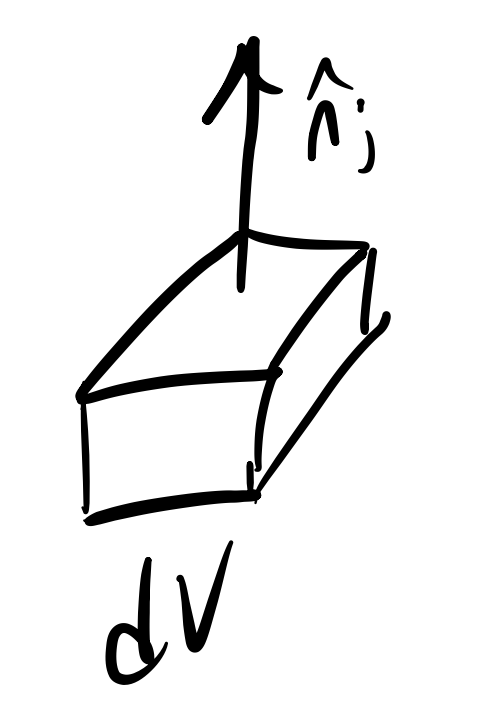
\includegraphics[scale=0.35]{Lectures/Images/lec1-volelement.png}
\end{center}

Therein, $\sigma_{ij}$ is the linear momentum flux, or a rank-2 stress tensor. Note that throughout, we use Einstein summation convention where repeated indices are summed over (e.g. $u_{ij}x_j \coloneqq \sum_j u_{ij}x_j$).

We can further write:
\begin{equation}
    f_i = \iiint \dpd{\sigma_{ij}}{x_j}dV
\end{equation}
Another way to package this; we can write the force as a volume integral of a force density, which is a divergence of the stress tensor:
\begin{equation}
    f_i = \iiint dV F_i
\end{equation}
with:
\begin{equation}\label{eq:forcedensity}
    \boxed{F_i = \p_j \sigma_{ij}}
\end{equation}
one can also take this as the definition of the stress tensor. If you have never seen the stress-tensor, it is recommended you read the first chapter of Soft Matter.

There is an assumption we made here. When we set the volume integral of $dVP_i$ equal to the area integral, we assumed that there were no sources. We will see what happens soon when this assumption is violated. For example we may have a solid immersed in a fluid, in which case Newton's third law may not hold and linear momentum is generically not conserved. One thing that this class will emphasize is what happens to the conclusions when assumptions are challenged!

Let's look at a differential of the force density:
\begin{equation}
    dF_i = \sigma_{ij}n_j dA
\end{equation}
As a concrete example, we can look at the forces acting on different faces of our cube:

\begin{center}
    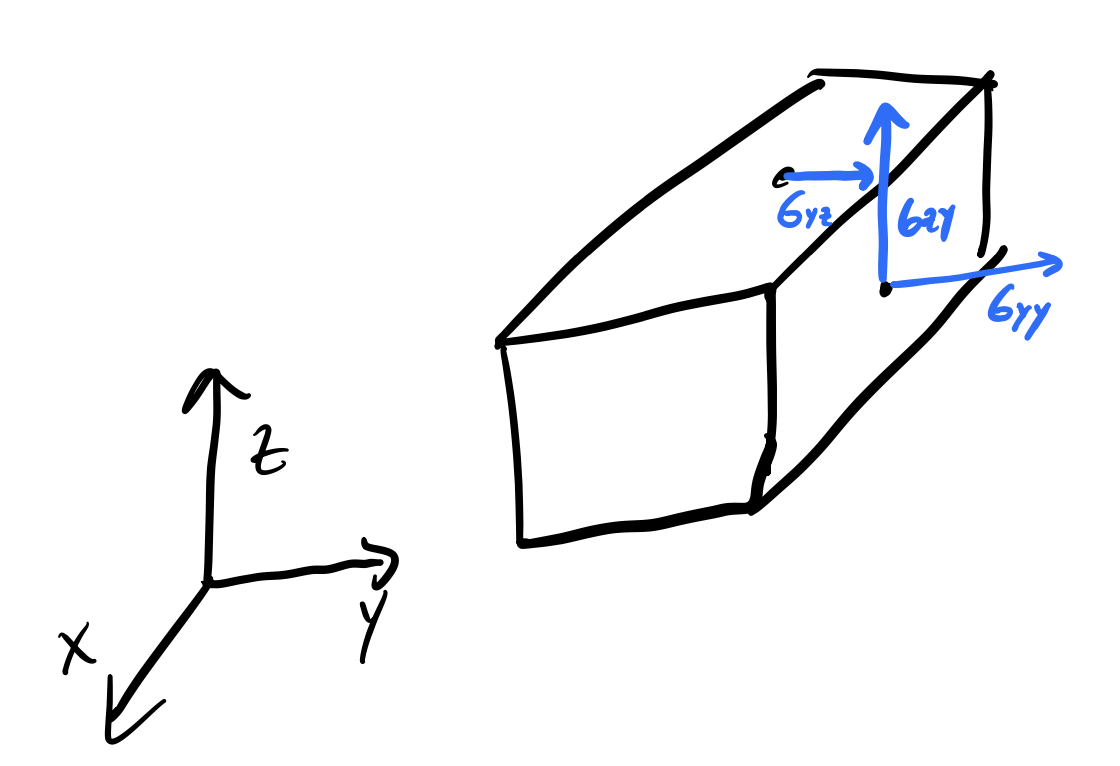
\includegraphics[scale=0.35]{Lectures/Images/lec1-forces.png}
\end{center}

\subsection{Constitutive Equation and Conservation Laws}
We want a relationship between the stress tensor and the order parameter, relating to the displacements. We assume that there is translation invariance for now, so there is no dependence on the displacements themselves, only on gradients of the displacements (this is not true always, e.g. in the case of a solid in fluid, or a solid on a table with glue - these will be additional terms that we consider later). In linear response theory, we connect the stress and strain tensors (rank-2) via a stiffness tensor (rank-4):
\begin{equation}
    \sigma_{ij} = K_{ijkl}\p_k u_l = K_{ijkl}u_{kl}
\end{equation}
The above is a linearized constitutive equation. As ugly as the $K_{ijkl}$ above may be, forms the identity of the material. This is ``Hooke's Law on steroids''. Note that if we assume that microscopically a solid is composed of masses connected by Hookian springs with spring constant $k$, it is possible to derive the macroscopic stiffness tensor from the microscopic theory; this may be one of your problems later.

In 2-D, we have:
\begin{equation}
    u_{kl} = \m{\p_x u_x & \p_x u_y \\ \p_y u_x & \p_y u_y}
\end{equation}
\begin{equation}
    \sigma_{ij} = \m{\sigma_{xx} & \sigma_{xy} \\ \sigma_{yx} & \sigma_{yy}}
\end{equation}
Note that we do not symmetrize here. In fact we can explicitly think about what happens in the cases when the off-diagonal entries are not equal. When $\sigma_{ij} \neq \sigma_{ji}$, it means that there is a non-vanishing net-torque (imagine back to the forces on the cube picture) and so the medium can spontaneously rotate. What does this teach us? Buried in the cumbersome algebraic structure of the rank-4 tensor, we see the presence and or violation of conservation laws. In this case, $\sigma_{ij} \neq \sigma_{ji}$ it implies that angular momentum is \emph{not} conserved. Most books assume the fundamental conservation laws of nature hold and write down theories accordingly. But, we can allow for exotic mechanisms of the breaking of such fundamental laws, e.g. from interactions with external sources which give rise to effective theories.

We are rapidly marching through conservation laws; we have imposed conservation of linear momentum from the get-go, but we do not impose $\sigma_{ij} = \sigma_{ji}$/impose angular momentum conservation (If we did, then the rank-4 tensor would reduce to rank-3). This means that we have external torques present/sources of angular momentum. As we go on, we will study symmetries of our system through the symmetries of the (admittedly complicated) $K_{ijkl}$ object, and understand the conservation laws through it.

Now, we \emph{assume} that there is a potential energy. In Hooke's law, we assume $F = -\p_x E$ with $E = \frac{1}{2}kx^2$ so we have a conservative force. Here, we don't work on the level of single particles, so we write the total potential energy as the integral over energy density:
\begin{equation}
    U = \iiint d^3x \e(\v{x})
\end{equation}
The question is now what is $\e(\v{x})$? If we want a linear force, we require that $\e(\v{x})$ be a quadratic form in $\v{x}$:
\begin{equation}
    \e(\v{x}) = \frac{1}{2}c_{ijkl} u_{ij}(\v{x})u_{kl}(\v{x})
\end{equation}
Now, we want the force in the $l$th direction, which is a functional derivative of the energy density:
\begin{equation}
    \left(\text{Force}\right)_l = -\frac{\delta \e}{\delta u_l} = -\left(\dpd{\e}{u_l} - \p_k \dpd{\e}{u_{lk}}\right)
\end{equation}
where again we recall $u_{lk} = \p_l u_k$. Let's try to unweird this expression via analogy (maybe you want to explain to a friend, or pick up someone at a bar by telling them that you work on functional derivatives) - in classical mechanics, we have an action:
\begin{equation}
    S = \int L(q(t))dt
\end{equation}
we then have the trajectory that is followed is that for which the functional derivative of the action vanishes\footnote{Of course, this is something your date is expected to know.}:
\begin{equation}
    \frac{\delta S}{\delta q} = 0 \implies \dpd{L}{q_j} - \dod{}{t}\left(\dpd{L}{\dot{q}_i}\right) = 0
\end{equation}
And we can now see that the form of this expression is equivalent to the functional derivative of the energy density we wrote above.

Since we that the energy density cannot depend on displacement $u_l$/it only depend on gradients of displacement; hence the first term of the force expression vanishes:
\begin{equation}
    \left(\text{Force}\right)_l = \p_k \dpd{\e}{u_{lk}}
\end{equation}
Now if we recall Eq. \eqref{eq:forcedensity} that the force density is the divergence of the stress tensor, we can write the above as:
\begin{equation}
    \sigma_{lk} = \dpd{\e}{u_{lk}}
\end{equation}
Now, if $\e$ is quadratic in $u$, we will find that the relationship of stress and strain will be linear. The question then becomes; what is the relationship between $K_{ijkl}$ and between $c_{ijnm}$ (the coefficients of force and the coefficients of energy)? In the Hooke's law case they coincide and are both the spring constant $k$. However, this coincidence is only because we have a conservative force - we will see that even in this more general/continuum setting that if we have energy conservation the coefficients coincide, and in non-conservative settings they may differ.

Let us work through the algebra. Computing the derivative of $\e$:
\begin{equation}
    \begin{split}
        \dpd{\e}{u_{pq}} &= \frac{1}{2}c_{ijkl}\left[\delta_{ip}\delta_{jq}u_{kl} + u_{ij}\delta_{pk}\delta_{ql}\right] 
        \\ &= \frac{1}{2}\left[c_{pqkl}u_{kl} + c_{ijpq}u_{ij}\right]
        \\ &= \frac{1}{2}\left[c_{pqkl}u_{kl} + c_{klpq}\right]u_{kl}
    \end{split}
\end{equation}
Note in the third equality we replace $ij$ with $kl$; they are dummy/repeated/summed over indices and thus we can call them whatever we want\footnote{Name-calling is not good, but its ok with tensors - they don't mind.}. Now, identifying:
\begin{equation}
    K_{pqkl} = \frac{1}{2}[c_{pqkl} + c_{klpq}]
\end{equation}
we have:
\begin{equation}
    \sigma_{pq} = K_{pqkl}u_{kl}
\end{equation}
And thus we manifestly see that the stiffness tensor is symmetric under interchange of pairs of indices, so long as the force is derived from a variation of a quadratic energy density:
\begin{equation}
    \boxed{K_{pqkl} = K_{klpq}}
\end{equation}
This relation is known as the Maxwell-Betti reciprocity. Later we will identify $\alpha \coloneqq pq$ and $\beta \coloneqq kl$ and better appreciate the symmetry algebraically.

\subsection{Non-Conservative Forces}
What if we have a world where we deform the material and through interaction with the environment, the system can suck up or expel energy? Then, we will find that work is not a state function, and:
\begin{equation}
    \oint \v{F} \cdot d\v{l}\neq 0 
\end{equation}
In this context, the linear stress-strain relation says \emph{nothing} about the conservative nature of the forces, only that the forces are linear. It only says something about the energy with the constraint that the forces are conservative.

How do we think about the tensors in this setting? Recall that we can always write a tensor in terms of a symmetric and antisymmetric part, e.g.:
\begin{equation}
    \sigma_{ij} = \sigma_{ij}^S + \sigma_{ij}^A
\end{equation}
with:
\begin{equation}
    \sigma_{ij}^S = \frac{\sigma_{ij} + \sigma_{ji}}{2}, \quad \sigma_{ij}^S = \sigma_{ji}^S
\end{equation}
\begin{equation}
    \sigma_{ij}^A = \frac{\sigma_{ij} - \sigma_{ji}}{2}, \quad \sigma_{ij}^A = -\sigma_{ji}^A
\end{equation}
here $\sigma_{ij}^S$ conserves angular momentum, and the antisymmetric part is the culprit of angular momentum conservation violation. Next class, we will do a similar decoupling for our stiffness tensor:
\begin{equation}
    K_{ijkl} = K_{ijkl}^e + K_{ijkl}^o
\end{equation}
with:
\begin{equation}
    K_{ijkl}^e = K_{klij}^e
\end{equation}
\begin{equation}
    K_{ijkl}^o = -K_{klij}^o
\end{equation}
the odd/o part will be new moduli that emerge only when our system is open/not closed. The existence of this term is known as odd elasticity. This subject started in 2020, from a Nature Physics paper first authored by a grad student here! This is not just a mathematical possibility, but indeed appears in nature, e.g. in chiral tissues.

Next time, we will understand these tensors via group theory. We will then see what the operational meanings of the tensors are. We will discuss what predictions we can make given a set of symmetries and conservation laws. 
\section{Classification/Constraints of Elastic Moduli}
For a less detailed discussion of what we discuss here, you can consult chapter 9 (``Active Matter'') of the Soft Matter textbook.

\subsection{Summary of Last Lecture}
Last lecture, we studied solids, and the relationship between the stress and strain tensor:
\begin{equation}
    \sigma_{ij} = K_{ijkl}\underbrace{u_{kl}}_{\p_k u_l}
\end{equation}
the two are related via the stiffness tensor $K_{ijkl}$, which summarizes the identity of the solid.

If the forces are conservative, then the stress is the variation of an energy density:
\begin{equation}\label{eq:sigmavariation}
    \sigma_{ij} = \dpd{\e}{u_{ij}}
\end{equation}
And it follows that $K_{ijkl}$ is symmetric under exchange of pairs of indices:
\begin{equation}\label{eq:reciprocity}
    K_{ijkl} = K_{klij}
\end{equation}

But, say we want to consider a medium where the forces are not conservative. Then neither of Eq. \eqref{eq:sigmavariation}, \eqref{eq:reciprocity} have to hold. In this more general case, we can split $K_{ijkl}$ into an even and odd part:
\begin{equation}
    K_{ijkl} = K^e_{ijkl} + K^o_{ijkl}
\end{equation}
where even/odd means that the tensor acquires a $\pm$ sign under swap of pairs of indices. In a soft matter or elasticity course you have seen the first term - but the second term is novel, and comes up when we study open systems.

Since the forces are non-conservative, work is no longer a state function:
\begin{equation}
    W_{AB} \neq U_B - U_A
\end{equation}
\begin{center}
    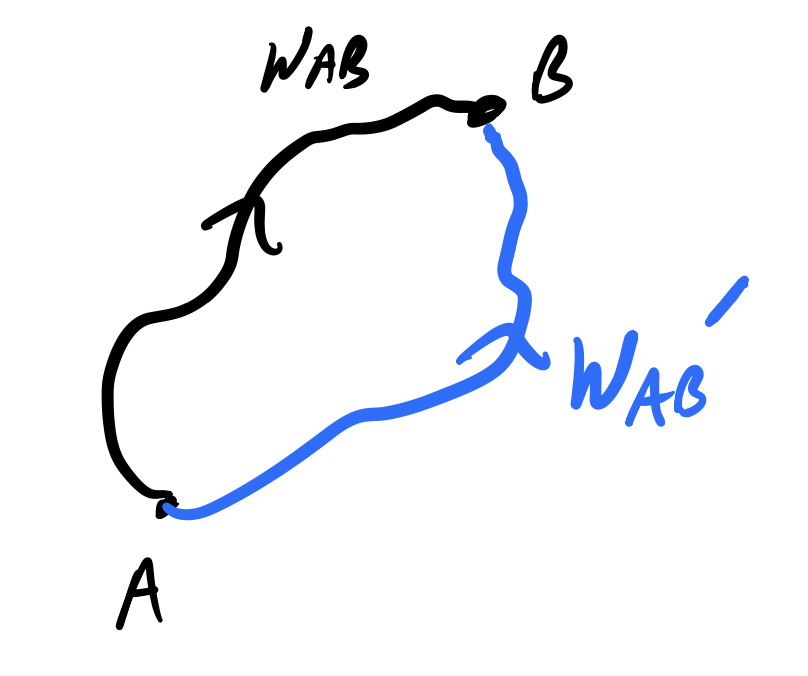
\includegraphics[scale=0.3]{Lectures/Images/lec2-work.png}
\end{center}
In this case, we have net work (positive or negative, depending on the sign) when we go around a cycle. The work done is rate-independent (no time derivatives here!). Further, the medium must be chiral because there is a difference in the sign of work depending on whether we traverse a loop clockwise or counterclockwise.

\subsection{Representations of Stress/Strain Tensors}
Let's try to classify all possibel entries of the stiffness tensor $K_{ijkl}$ using the representations of $\sigma$ and $u$; this will allow us to classify possible elastic moduli. In particular, let us try to classify odd elasticity $K^o_{ijkl}$ in 2-dimensions. In 2-D, stress $\sigma_{ij}$ and strain $u_{kl}$ each have 4-independent components, which we may package into a 4-entry vector. Therein the stiffness $K_{\alpha\beta}$ is a 4x4 matrix that connects them. We ``play God'' by analyzing/studying the form of $K_{\alpha\beta}$ without knowing any details about our system - we can deduce constraints purely mathematically.

\begin{center}
    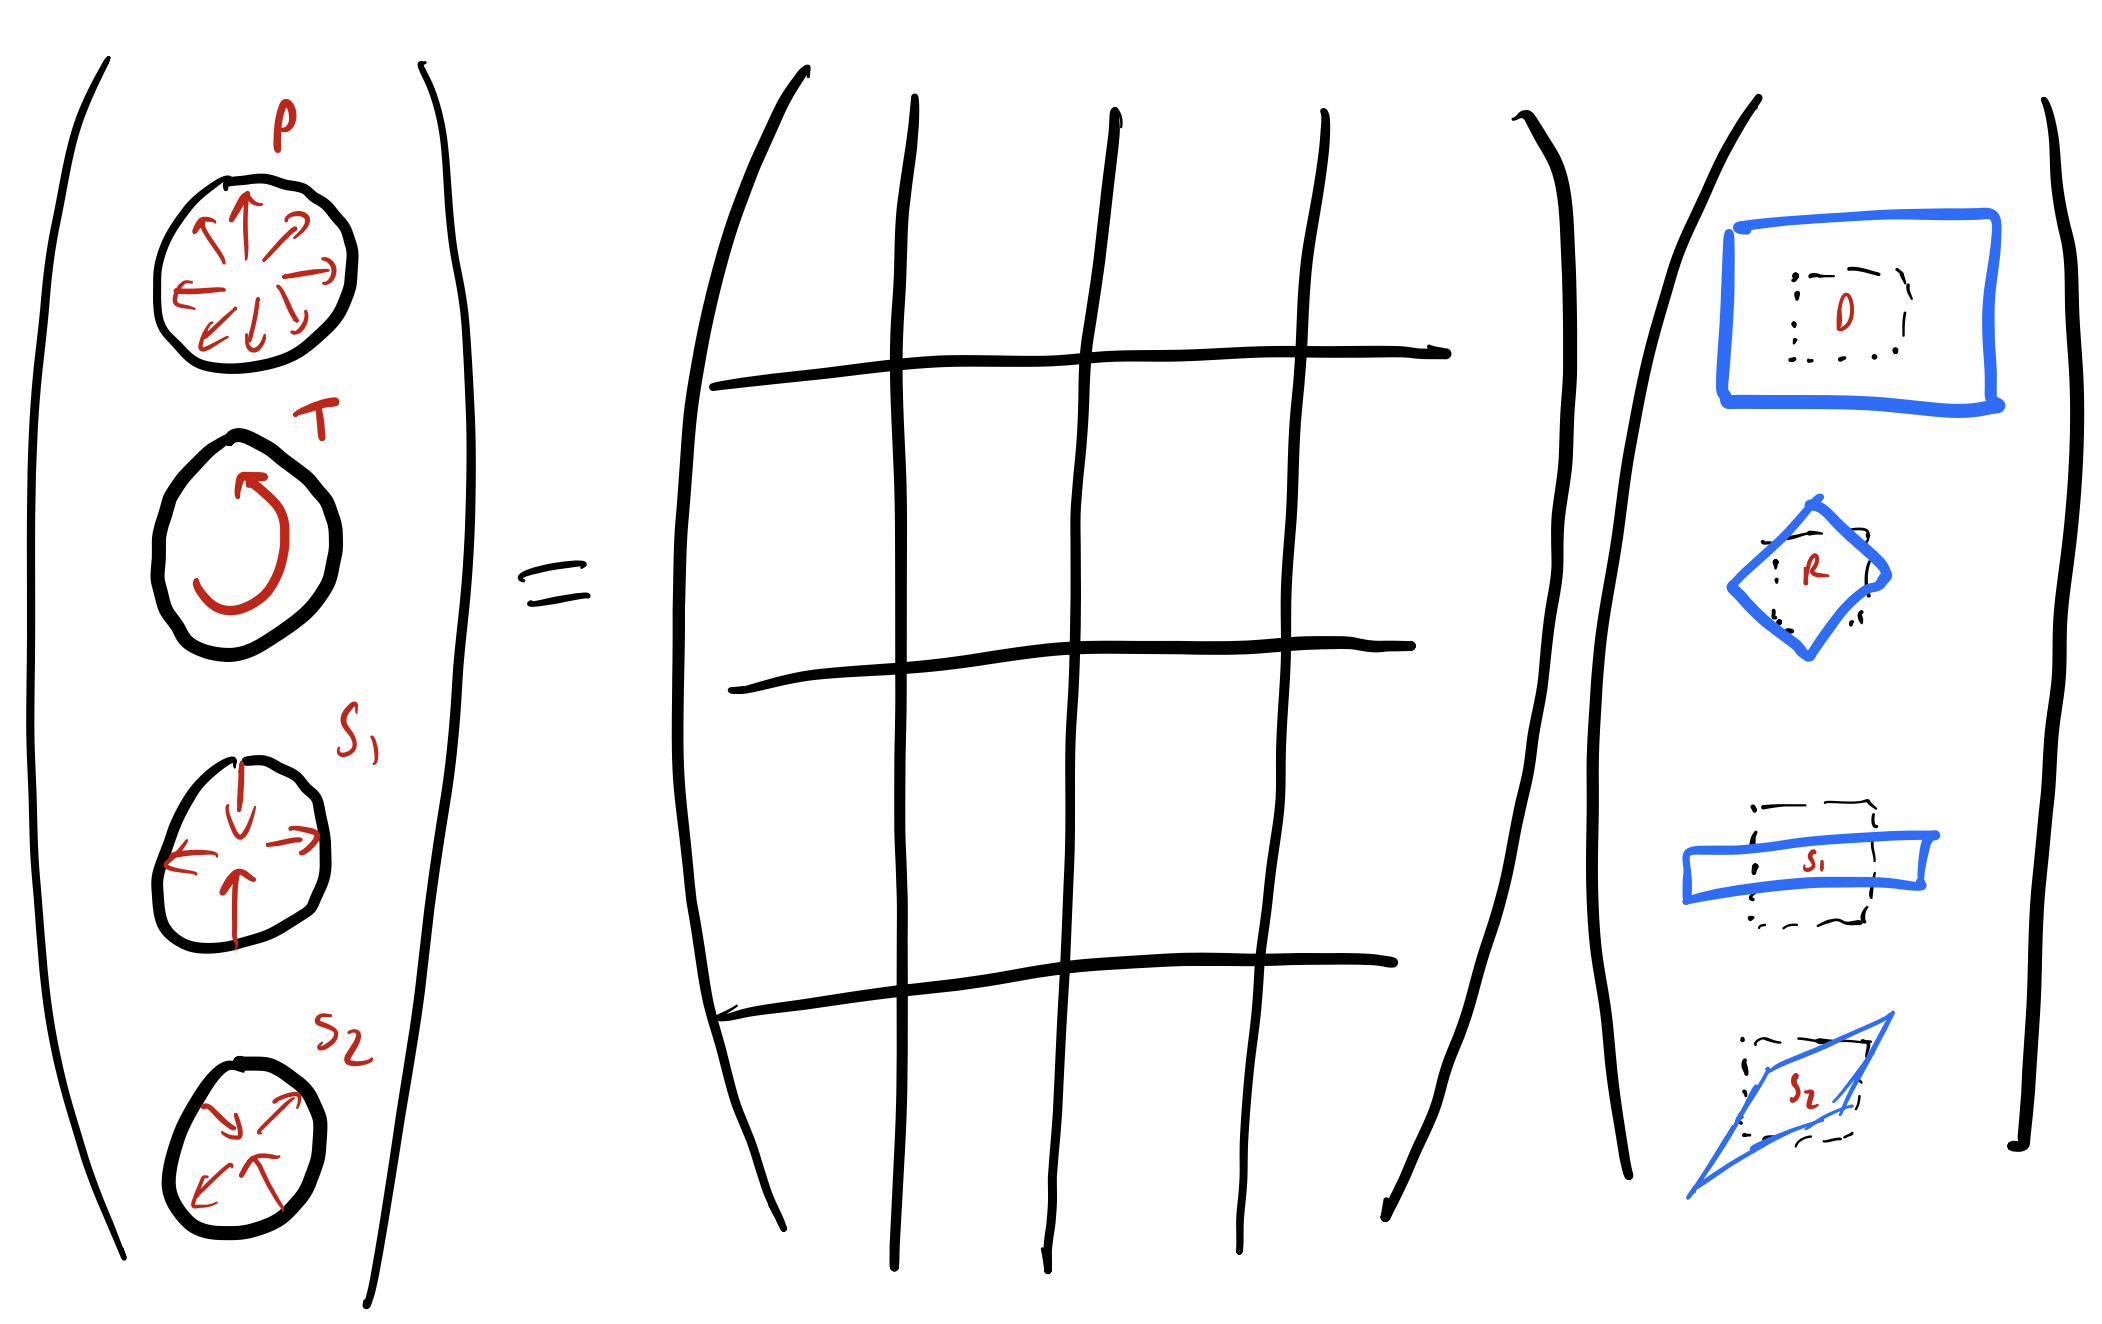
\includegraphics[scale=0.35]{Lectures/Images/lec2-stiffnessmatrix.png}
\end{center}
\begin{equation}
    \m{\text{P} \\ \text{T} \\ \text{SS1} \\ \text{SS2}} = \m{\cdot & \cdot & \cdot & \cdot \\ \cdot & \cdot & \cdot & \cdot \\ \cdot & \cdot & \cdot & \cdot \\ \cdot & \cdot & \cdot & \cdot}\m{\text{D} \\ \text{R} \\ \text{S1} \\ \text{S2}}
\end{equation}

The four entries of strain $u_{\beta}$ will be the projections onto the basis elements of dilation, rotation, 2 shears. We can do the same for stress, writing down the forces that result from the deformations - pressure, torque, and shear stress 1/2. Then the matrix elements of $K_{\alpha\beta}$ relate the two.

What is the analytical meaning of the drawings above? We write:
\begin{equation}
    u_{ij} = \sum_{\alpha=0}^3 u^\alpha \tau_{ij}^\alpha
\end{equation}
with:
\begin{equation}
    \tau^0 = \m{1 & 0 \\ 0 & 1}, \quad \tau^1 = \m{0 & 1 \\ -1 & 0}, \quad \tau^2 = \m{1 & 0 \\ 0 & -1}, \quad \tau^3 = \m{0 & 1 \\ 0 & 1}
\end{equation}
Corresponding to dilation, rotation, shear 1, and shear 2 respectively. Note that these obey the relation (note that we take a trace below, since the indices are repeated and hence summed):
\begin{equation}
    \boxed{\tau_{ij}^\alpha \tau_{ij}^\gamma = 2\delta^{\alpha\gamma}}
\end{equation}
This is the algebra for the generators of the rotation group in 2-D.

This was a statement about the geometry of the strain deformation. We can do a similar procedure for the stress:
\begin{equation}
    \sigma_{ij} = \sum_{\alpha=0}^3 \sigma^\alpha \tau^\alpha_{ij}
\end{equation}
where now the projections onto $\tau^0, \tau^1, \tau^2, \tau^3$  correspond to pressure, torque, shear stress 1, shear stress 2.

\subsection{Classifying elastic moduli}
Now, we want to discover what is in the $K_{\alpha\beta}$ matrix. To this end, we can think about symmetries of the medium. One such symmetry/idea is isotropy - wherein there is no preferred direction to the material. With this assumption we can already set a lot of the entries of $K$ to zero. 

In a world that is isotropic, I cannot couple a scalar/pseudoscalars to a vector/bivectrs - why? Because this would involve a preferred direction. So, look at the matrix element of $K$ that connects dilation with shear stress. We cannot measure the angle of shear in a isotropic medium, so this matrix element must vanish.

More generally, the dilation/rotation subspaces are scalar/pseudoscalars, and the stress subspaces are pseudovectors. Further, pressure/torque are scalar/pseudoscale and shear stress are pseudovector. By isotropy the subspaces cannot be connected, which allows us to conclude that 8 of the entries vanish:

\begin{equation}
    \m{\text{P} \\ \text{T} \\ \text{SS1} \\ \text{SS2}} = \m{\cdot & \cdot & 0 & 0 \\ \cdot & \cdot & 0 & 0 \\ 0 & 0 & \cdot & \cdot \\ 0 & 0 & \cdot & \cdot}\m{\text{D} \\ \text{R} \\ \text{S1} \\ \text{S2}}
\end{equation}

Next, consider the symmetry of objectivity/frame invariance. We can consider the solid to be ``self-standing'' - in this case, applying a rigid body rotation applies no stress. Note that we can break this if the solid was standing on some sticky surface (in which case we could have stresses applied from the contact) - symmetries can be broken by perturbations, e.g. isotropy via a magnetic field. But what does this frame invariance give us for the stiffness tensor? Since rotation generates no stresses, the entire second column is set to zero (rotations cannot generate pressure or torques).

\begin{equation}
    \m{\text{P} \\ \text{T} \\ \text{SS1} \\ \text{SS2}} = \m{\cdot & 0 & 0 & 0 \\ \cdot & 0 & 0 & 0 \\ 0 & 0 & \cdot & \cdot \\ 0 & 0 & \cdot & \cdot}\m{\text{D} \\ \text{R} \\ \text{S1} \\ \text{S2}}
\end{equation}

We have assumed that linear momentum is conserved. We have not used energy conservation here - let's see what this implies for us now.

To learn about the last remaining entries, let us work through some algebra. We write:
\begin{equation}
    \sigma_{ij} = \textcolor{blue}{\sigma^\gamma \tau^\gamma_{ij}} = K_{ijkl} = u_{kl} = \textcolor{blue}{K_{ijkl}\tau^\beta_{kl}u^\beta}
\end{equation}
Now multiplying the blue by $\frac{1}{2}\tau^\alpha_{ij}$, then on the LHS I get:
\begin{equation}
    \frac{1}{2}\tau^\alpha_{ij}\sigma^\gamma \tau^\gamma_{ij} = \frac{1}{2}\sigma^\gamma 2\delta^{\alpha\gamma} = \sigma^\alpha
\end{equation}
and on the RHS we get:
\begin{equation}
    \frac{1}{2}\tau^\alpha_{ij} K_{ijkl}\tau^\beta_{kl}u^\beta
\end{equation}
so:
\begin{equation}
    \sigma^\alpha = \frac{1}{2}\tau^\alpha_{ij} K_{ijkl}\tau^\beta_{kl}u^\beta = K^{\alpha\beta}u^\beta
\end{equation}
So, if we assume that the theory is conservative/we have reciprocity $K_{ijkl} = K_{klij}$, then $K^{\alpha\beta} = K^{\beta\alpha}$ - the matrix is symmetric, and so we can set the matrix element that connects dilation to torque is zero:
\begin{equation}
    \m{\text{P} \\ \text{T} \\ \text{SS1} \\ \text{SS2}} = \m{\cdot & 0 & 0 & 0 \\ 0 & 0 & 0 & 0 \\ 0 & 0 & \cdot & \cdot \\ 0 & 0 & \cdot & \cdot}\m{\text{D} \\ \text{R} \\ \text{S1} \\ \text{S2}}
\end{equation}
We can name some of the remaining entries; the entry connecting dilation to pressure is the bulk modulus $B$:
\begin{equation}
    \m{\text{P} \\ \text{T} \\ \text{SS1} \\ \text{SS2}} = \m{B & 0 & 0 & 0 \\ 0 & 0 & 0 & 0 \\ 0 & 0 & \cdot & \cdot \\ 0 & 0 & \cdot & \cdot}\m{\text{D} \\ \text{R} \\ \text{S1} \\ \text{S2}}
\end{equation}
Now, it is an exercise that you may have on a problem set that isotropy constrains the lower diagonal entries to be the same, and the lower off-diagonal entries to be equal and opposite. The diagonals we can call the shear modulus $G$, and the off-diagonals must be zero (as energy conservation constrains $K^{\alpha\beta}$ to be symmetric). Thus:
\begin{equation}
    \m{\text{P} \\ \text{T} \\ \text{SS1} \\ \text{SS2}} = \m{B & 0 & 0 & 0 \\ 0 & 0 & 0 & 0 \\ 0 & 0 & G & 0 \\ 0 & 0 & 0 & G}\m{\text{D} \\ \text{R} \\ \text{S1} \\ \text{S2}}
\end{equation}

So, if we assume isotropy, frame invariance, and conservative forces, we just have $B, G$ above. Let's repeat the analysis if we do not assume conservative forces. The diagonal components are not affected, but the off-diagonal entries we constrained to be zero are now generically nonzero:
\begin{equation}
    \m{\text{P} \\ \text{T} \\ \text{SS1} \\ \text{SS2}} = \m{B & 0 & 0 & 0 \\ A & 0 & 0 & 0 \\ 0 & 0 & G & -K^0 \\ 0 & 0 & +K^0 & G}\m{\text{D} \\ \text{R} \\ \text{S1} \\ \text{S2}}
\end{equation}

So, this is the conclusion of our analysis - we have (relaxing energy conservation) 4 moduli describing our material. 

Comment: In an anisotropic medium, we could have the moduli coupling the two shears, but they will \emph{not} be equal and opposite. One could then imagine matrix elements of the form $\e + K^0, \e - K^0$; one must look at the \emph{difference} to conclude nonconservative forces (just looking at one element, you cannot be sure if the source is anisotropy). Additionally, a nonzero $A$ does not necessarily mean nonconservative forces, it means nonconservative forces \emph{and} frame invariance, so to conclude nonconservative forces concretely we would need to compare with the other matrix element across the diagonal.

\subsection{Quantifying Work}
We derive the expression for the work coming from the stresses. For a force we have the contour integral:
\begin{equation}
    W = -\oint \v{F} \cdot d\v{l}
\end{equation}
For stresses, we consider a loop integral in 4-D space:
\begin{equation}
    W = -\oint \sigma_{ij}du_{ij} = -\oint \sigma^\beta du^\beta
\end{equation}
Now using Stokes' theorem:
\begin{equation}
    W = \iint \e^{\alpha\beta}\frac{\partial \sigma^\beta}{\partial u^\alpha}dA
\end{equation}
With $\e^{\alpha\beta} = \m{0 & -1 \\ 1 & 0}$. Now, we can use that $\sigma^\beta = K^{\beta\alpha}u^\alpha$, and take the derivative. Note that we can focus solely on the entries of the tensor coming from the non-conservative forces (the parts coming from conservative forces give trivially zero contribution)! Writing $K^{\alpha\beta} = K^0e^{\alpha\beta}$ (we focus on the subspace of shears), we get:
\begin{equation}
    W = -\iint \e^{\alpha\beta}e^{\beta\alpha}K^0 dA
\end{equation}
Then:
\begin{equation}
    \e^2 = \m{-1 & 0 \\ 0 & -1} \implies -\e^{\alpha\beta}e^{\beta\alpha} = 2
\end{equation}
and so:
\begin{equation}
    W = 2K^0 \cdot \text{Area}
\end{equation}
So we see that we do indeed have a nonzero amount of work, proportional to the odd elastic modulus and enclosed area.
\section{Microscopic Sources of Exotic Stiffness}

\subsection{Review}
Last time, we tried to constrain the stiffness tensor:
\begin{equation}
    \sigma^\alpha = K^{\alpha\beta}u^\beta
\end{equation}

Assuming isotropy, the subspaces of scalars and vectors could not be connected (so the off diagonal blocks vanish), and assuming frame invariance, rotations cannot generate any stresses, so:
\begin{equation}
    \m{\text{P} \\ \text{T} \\ \text{SS1} \\ \text{SS2}} = \m{\cdot & 0 & 0 & 0 \\ \cdot & 0 & 0 & 0 \\ 0 & 0 & \cdot & \cdot \\ 0 & 0 & \cdot & \cdot}\m{\text{D} \\ \text{R} \\ \text{S1} \\ \text{S2}}
\end{equation}
Isotropy further contains that the lower diagonals are the same and lower off diagonals are the same, so the most general form of the tensor is:
\begin{equation}\label{eq:macroscopic}
    \m{\text{P} \\ \text{T} \\ \text{SS1} \\ \text{SS2}} = \m{B & 0 & 0 & 0 \\ A & 0 & 0 & 0 \\ 0 & 0 & G & -K^0 \\ 0 & 0 & +K^0 & G}\m{\text{D} \\ \text{R} \\ \text{S1} \\ \text{S2}}
\end{equation}
Important point - the existence of the odd elastic moduli $K^0$ implies two things. First, the structure of the theory is non-variational; we can go around quasi-statically in the space of strains, and we find the work is nonzero:
\begin{equation}
    W = \oint \sigma_{ij}du_{ij}\neq 0
\end{equation}
This tells us that there is a chirality in the material (this was also manifest from the fact that - if $G = 0$, then the part of the stiffness matrix acting on the shear subspace looks like $K^0\e$). Another clear manifestation of chirality is if $A \neq 0$, in which case we can have torques (note - no angular momentum conservation!) as a result of dilations.

\subsection{Non-reciprocal gadget and constructions}
This is an example of a $K^0 \neq 0, A = 0$ system from a recent Nature paper \texttt{Veenstra, Scheibner, Brandenbourger, Binysh, Souslov, Vitelli, Coulais. \emph{Nature} (2025)}. As warm-up, consider the following spring system:

\begin{center}
    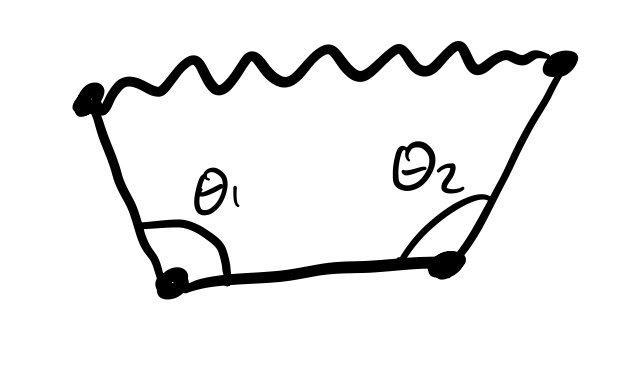
\includegraphics[scale=0.35]{Lectures/Images/lec3-gadgetwithspring.png}
\end{center}

If we have a bond-bending interaction, we have a bond-bending stiffness:
\begin{equation}
    \m{\tau_1 \\ \tau_2} = \m{-\kappa & \kappa^s \\ \kappa^s & -\kappa}\m{\delta\theta_1 \\ \delta\theta_2}
\end{equation}
where the diagonals come from the bond-bending, and the off-diagonals (symmetric!) come from the coupling spring. For this system:
\begin{equation}
    \nabla \times \gv{\tau} = \v{0}
\end{equation}
but we can introduce batteries/motors to break this symmetry. If Maxwell-Betti reciprocity is obeyed, then pushing one side of the object should repel the other symmetrically. But we can introduce motors to make this building block non-reciprocal; pressing on the left side the right side repels, pressing on the right side the left side \emph{attracts}.
\begin{center}
    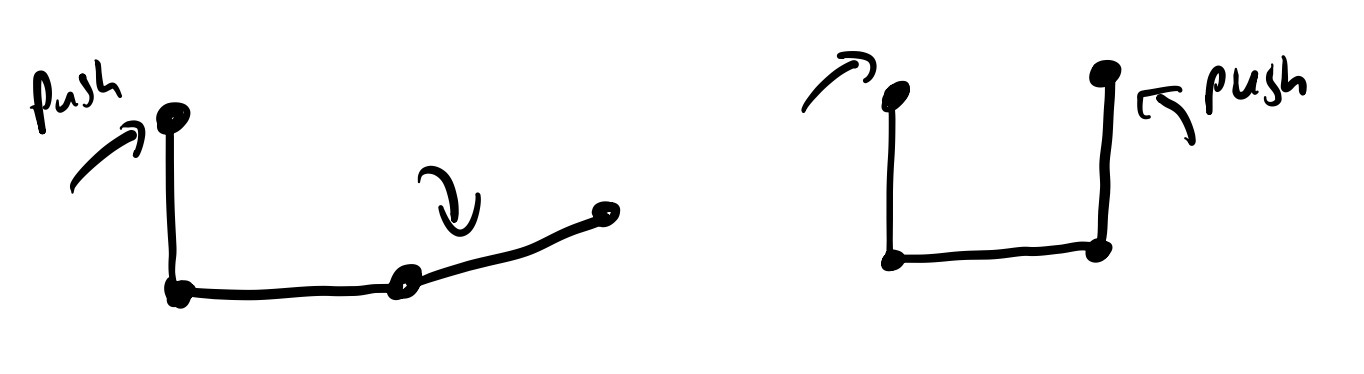
\includegraphics[scale=0.35]{Lectures/Images/lec3-nonreciprocalgadget.png}
\end{center}
This means that we have a stiffness tensor of the form:
\begin{equation}\label{eq:microscopic}
    \m{\tau_1 \\ \tau_2} = \m{-\kappa & -\kappa^a \\ \kappa^a & -\kappa}\m{\delta\theta_1 \\ \delta\theta_2}
\end{equation}

A technical comment - notice that the interaction we've written above is a striking example of a non-pairwise interaction. The torque at point 1 doesn't just depend on the pair of rods eminating out of it, but also from the other components of the system.

What is the physical consequence of this non-reciprocal interaction? Now, we can go through a cycle and generate non-zero work. If we make a ring of these objects - with the motors off, the system jiggles a bit before being slowed to rest with friction. With the motors on, we perturb the medium and in trying to undo the deformation/get back to the starting point the motors can induce energies into the system and the system can keep jiggling forever (using the energy provided by the external motors).

If we think about the dynamics, we have:
\begin{equation}
    \m{I\delta \ddot{\theta}_1 \\ I\delta \ddot{\theta}_2} = \m{-\kappa & -\kappa^a \\ \kappa^a & \kappa}\m{\delta \theta_1 \\ \delta\theta_2}
\end{equation}
If we diagonalize to find the normal frequencies, we have:
\begin{equation}
    \omega^2 = \frac{\kappa}{I} \pm i\frac{\kappa^a}{I}
\end{equation}
The first term makes total sense - this is what we have for just a regular spring system that you've seen many times before in classical mechanics. But the antisymmetric term produces an imaginary component to $\omega^2$! This means that (in the absence of nonlinearities - we have assumed linear response for this whole discussion) we have unbounded growth/amplification of the motion! Of course building this gadget in real life we do in fact have nonlinearities - when the angles become large the components of the gadget can touch - which prevents unbounded growth.

Now, we can take our object - where the antisymmetric $\kappa^a$ breaks the chiral symmetry - and map out the dynamics in strain space (with the two shears being the two axes). The system can exhibit chaotic behaviour!

Let us ``rediscover'' the wheel (again, still composed of the the gadget). Original conception of a wheel has a circular, fixed shape which moves via force supplied to it from axle (via animal, motor etc.) But our new wheel is adaptive, and moves via deformations. It can come across a rough uphill landscape and use the deformations caused by the rough landscape to travel through it! In fact we can make the problem even harder - we can make a landscape of granular uphill matter, and our sophisticated wheel can still go up it (we can also flip the sign of $\kappa^a$ - we are allowed to pick/tune whatever sign for these - and it can travel the other way).

We can also build up a crystal out of this gadget by tiling. We can throw a projectile onto the crystal, which is then ejected back upwards at an angle (the angle/asymmetric response is expected! The medium is chiral. Again, we can flip the angle by flipping the sign of $\kappa^a$).

Motivating a homework problem you will do - there is a microscopic law Eq. \eqref{eq:microscopic} and the macroscopic/continuum description Eq. \eqref{eq:macroscopic}. Without calculation, we can deduce $K^0 \sim \kappa^a$ and $G \sim \kappa$. We can do a more detailed derivation and derive the macroscopic dependence on the microscopic parameters (and then check that this dependence works out in experiment)! In your homework, you will just take a normal (not odd!) hexagonal microscopic lattice, and see how the macroscopic properties/parameters and their dependencies emerge.

\subsection{Microscopic source of $A$}

If we have a central force, we can generically write things as a gradient of a potential. We introduce non-conservative forces in terms of a non-central part. Consider the spring:

\begin{center}
    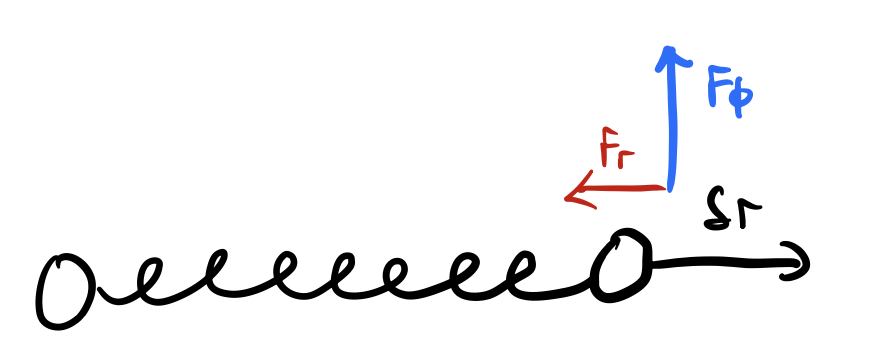
\includegraphics[scale=0.35]{Lectures/Images/lec3-noncentralspring.png}
\end{center}

\begin{equation}
    \v{F} = -(\kappa\hat{\v{r}} + \kappa^a\hat{\gv{\phi}})\delta r
\end{equation}
Or as a matrix equation:
\begin{equation}
    \m{F_r \\ F_\phi} = \m{-\kappa & 0 \\ -\kappa^a & 0}
\end{equation}
Notice again the crucial point - the off-diagonals are \emph{not} equal. This implies that:
\begin{equation}
    \oint \v{F} \cdot d\v{l} \propto \kappa^a
\end{equation}
(and does not vanish). The central part does not contribute to the net work as to the central part we can always prescribe a potential. Generally here, $\v{F} \neq -\nabla U$ so long as $\kappa^a \neq 0$. If we built up a lattice/continuum out of this microscopic piece, we could derive how the $A$ modulus emerges from the nonzero $\kappa^a$.

Let us consider a simple exercise - let's derive the work done in a cycle.

\begin{center}
    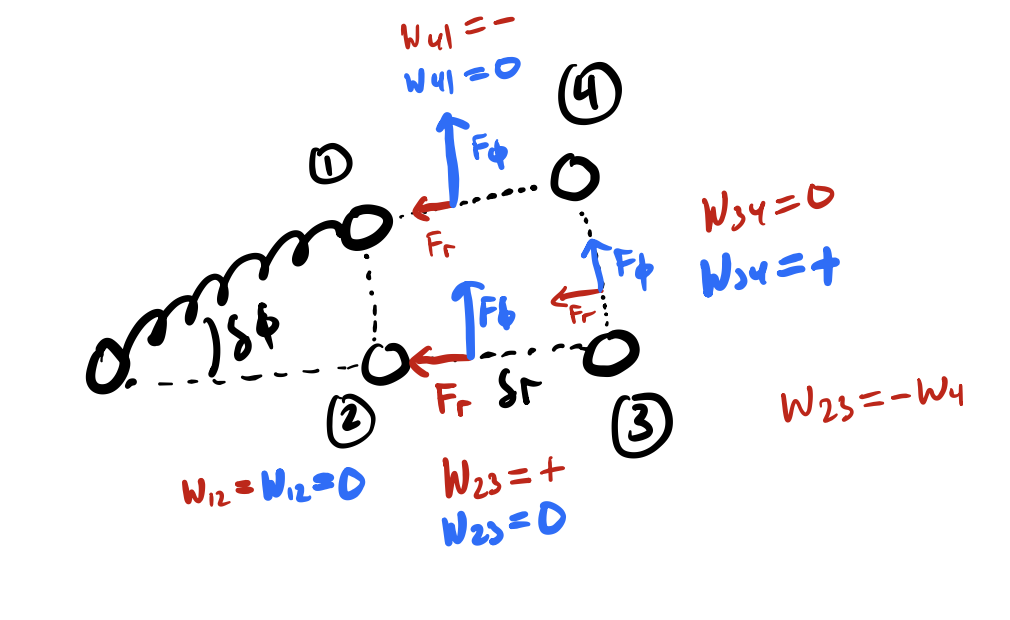
\includegraphics[scale=0.5]{Lectures/Images/lec3-noncentralspringwork.png}
\end{center}

\begin{itemize}
    \item From 1 to 2, there is no force and hence no work done.
    \item From 2 to 3, the direction of motion is radial, so only the radial component of the force contributes (positive) work.
    \item From 3 to 4, the direction of motion is tangential, so the tangential component of the force picks up (positive) work.
    \item From 4 to 1, the direction of motion is radial, so the radial component of the force contributes (negative) work. This work is equal and opposite to the work in step 2$\to$3.
\end{itemize}

Thus only surviving term is $W_{34}$ arising from $F_\phi$, which we can calculate to be:
\begin{equation}
    \oint \v{F} \cdot d\v{l} = W_{34} = F_\phi dl = \kappa^a \delta r (r + \delta r)\delta \phi \approx \kappa^a (r\delta \phi)\delta r = \kappa^a \cdot \text{Area}
\end{equation}

So in the harmonic approximation, with:
\begin{equation}
    F''(r) = F''(a) - \kappa(r - a), \quad F_\perp \approx F^\perp(a) - \kappa^a(r - a)
\end{equation}
we can derive the bulk and shear moduli:
\begin{equation}
    B = \frac{\sqrt{3}}{2}\left(\kappa + \frac{F''(a)}{a}\right), \quad G = \frac{\sqrt{3}}{4}\left(\kappa - 3\frac{F''(a)}{a}\right)
\end{equation}
as well as the $K^0/A$ moduli:
\begin{equation}
    A = -\frac{\sqrt{3}}{2}\left(\kappa^a - \frac{F^\perp(a)}{a}\right), \quad K^0 = \frac{\sqrt{3}}{4}\left(\kappa^a - 3\frac{F^\perp(a)}{a}\right)
\end{equation}
note that the precise dependence depends on not just the force mechanism but also the layout of the lattice (e.g. will change with hexagonal, square etc.). If we did a similar derivation with the non-reciprocal robot gadget, we could also derive a macro-from-micro result from above (see the paper!), with $A = 0$ and $K^0 \neq 0$.

\subsection{Other contemporary experiments}

There have been a number of recent experiments that measure interesting non-central crystals. For example colloidal spinners in a magnetic field that form odd elastic crystals \texttt{Bililign, Usabiaga, Ganan, Poncet, Soni, Magkiriadou, Shelley, Bartolo, Irvine. \emph{Nature} (2022)} or crystal formation in biological platforms \texttt{Tan, Mietke, Higinbotha, Li, Chen, Foster, Gokhale, Dunkel, Fakhri. \emph{Nature} (2022)}.

In such non-central crystals, there is the potential to measure lubrication forces:

\begin{center}
    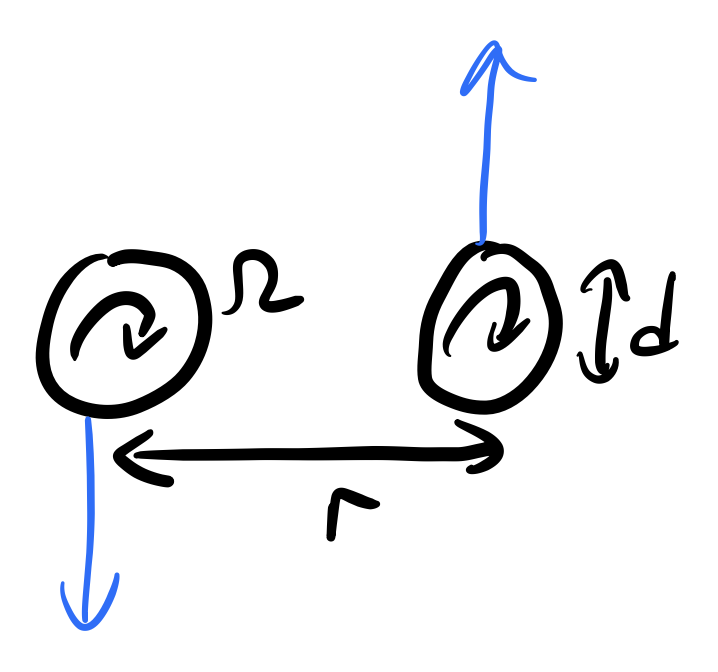
\includegraphics[scale=0.35]{Lectures/Images/lec3-lubricationforces.png}
\end{center}

where:
\begin{equation}
    F^\perp \propto \Omega \log\left(\frac{r - d}{d}\right)
\end{equation}

Next time - we will take the macroscopic theory, and study the stability of the lattice, as well as excitations (sound modes) in it. These have been concretely measured in robotic platform, and allegedly in the biological platform above (and perhaps possible to measure it in the colloidal spinner crystal?) however in the latter two cases the micro-to-macro correspondence is much well less understood.
\section{Odd Elastodynamics}

Last time, we looked at microscopic models where odd elasticity could arise. We also looked in detail at how energy could be generated in cycles of such system. Today we look odd elastodynamics, and study the dynamical equation for the displacement field. The presentation will be more algebraic.

In the last few lectures, we had pictures of different stresses/strains - these were pictorial representations of tensors, and in this lecture we make a dictionary to map between the pictures and algebra. For example we'll see how the tensors:
\begin{equation}
    \m{1 & 0 \\ 0 & 1} \to \delta_{ij}, \quad \m{0 & -1 \\ 1 & 0} \to \e_{ij}
\end{equation}
connect to stress/strain. For simplicity, we stay in 2D.

We recall the stress/strain relation:
\begin{equation}
    \sigma_{ij} = K_{ijmn}\p_m u_n  = K_{ijmn}u_{mn}
\end{equation}
Where we have the stiffness tensor $K_{ijmn}$. We wrote this relation (using symmetry constraints) as:
\begin{equation}\label{eq:macroscopic}
    \m{\text{P} \\ \text{T} \\ \text{SS1} \\ \text{SS2}} = \m{B & 0 & 0 & 0 \\ A & 0 & 0 & 0 \\ 0 & 0 & G & -K^0 \\ 0 & 0 & +K^0 & G}\m{\text{D} \\ \text{R} \\ \text{S1} \\ \text{S2}}
\end{equation}
Note that if $\sigma_{ij} = \frac{\delta \e}{\delta u_{ij}}$, then $K_{ijmn} = K_{mnij}$, but if $\sigma_{ij}$ is not of this form then $K$ is not necessary symmetric, so we can have the elastic moduli $K^0, A$ emerge in the stiffness tensor.

\subsection{Algebraic Representation of Stiffness Tensor}
Let's now switch to an algebraic representation:
\begin{equation}
    K_{ijmn} = B\delta_{ij}\delta_{mn} - A\e_{ij}\delta_{mn} + G(\delta_{in}\delta_{jm} + \delta_{im}\delta_{jn} - \delta_{ij}\delta_{mn}) + K^0 \frac{1}{2}(\e_{im}\delta_{jn} + \e_{in}\delta_{jm} + \e_{jm}\delta_{in} + \e_{jn}\delta_{im})
\end{equation}
The first term corresponds to the bulk modulus, which connects the dilation (projection of $u_{mn}$ onto identity/$\delta_{mn}$) and the pressure (projection of $\sigma_{ij}$ onto identity/$\delta_{ij}$). Thus it is not surprising that it has the form above; explicitly, they are derived via:
\begin{equation}
    P\delta_{ij} = B(\nabla \cdot \v{u})\delta_{ij} \implies \sigma_{ij} = \left[B\delta_{ij}\delta_{mn}\right]\p_m u_n
\end{equation}
For torque, we project $\sigma_{ij}$ onto the antisymmetric matrix $\e_{ij}$ (the sign of $A$ in $K_{ijmn}$ is up to convention of dilation - we choose it to be negative so we get a positive sign in the equation of motion):
\begin{equation}
    T\e_{ij} = A(\nabla \cdot \v{u})\e_{ij} \implies \sigma_{ij} = \left[A\e_{ij}\delta_{mn}\right]\p_m u_n
\end{equation}

Note that the $G$ term is invariant/same sign (even) under $ij \leftrightarrow mn$, while the $K^0$ term flips sign (odd) under $ij \leftrightarrow mn$.

\subsection{Equation of Motion}
I can now calculate the stress in terms of the strain, and taking one more derivative of the stress I can get the force. Then we obtain the equation of motion for odd elasticity!

\begin{equation}
    \rho \p_t^2 u_j + \Gamma \p_t u_j = F_j = \p_i \sigma_{ji} = \p_i (K_{jimn} \p_m u_n ) = K_{jimn}\p_i \p_m u_n
\end{equation}
where we note that the $\p_i$ commutes across the $K_{jimn}$ as the stiffness tensor is position independent (just a tensor of numbers). Thus, we have an EoM that relates a first + second time derivative to a second spatial derivative of displacement/strain.

If we looked at the robots of last time (centimeter scale), the first/inertial term $\rho \p_t^2 u_j$ is important. But for very small systems we can consider the overdamped limit (equivalently - the low Reynolds number\footnote{$R = \frac{uL}{\nu}$ with $u$ the velocity, $L$ the characteristic size, $\nu$ the viscosity} limit):
\begin{equation}
    \Gamma \dot{u}_j \gg \rho \ddot{u}_j.
\end{equation}
Thus, in the analysis of our equations of motion we neglect the inertial term.

A good exercise is to massage the derivatives until the terms with two spatial derivatives have recognizable form. For the $B$ term, we get:
\begin{equation}
    \Gamma \p_t u_j = \p_i K_{jimn} \stackrel{B-term}{=} \p_i B \delta_{ji}\delta_{mn}u_{mn} = B\p_j \p_i u_i
\end{equation}
or as a vector:
\begin{equation}
    \Gamma \p_t \v{u} = B\nabla(\nabla \cdot \v{u})
\end{equation}
For the $A$ term, we get:
\begin{equation}
    \Gamma \p_t u_j = \p_i K_{jimn} \stackrel{A-term}{=} A\e_{ji}\delta_{mn}\p_i u_{mn} = A\e_{jk}\p_k \p_i u_i
\end{equation}
or as a vector:
\begin{equation}
    \Gamma \p_t \v{u} = A\zhat \times \nabla(\nabla \cdot \v{u})
\end{equation}

Writing down the other terms:
\begin{equation}
    \Gamma \p_t u_j = B\nabla(\nabla \cdot \v{u}) + G\nabla^2u_j + A\e_{jk}\p_k \p_i u_i + K^0\e_{jk}\nabla^2 u_k 
\end{equation}
or vectorially:
\begin{equation}
    \Gamma \p_t \v{u} =B\nabla(\nabla \cdot \v{u}) + G\nabla^2\v{u} + A\zhat \times \nabla(\nabla \cdot \v{u}) + K^0 \zhat \times (\nabla^2 \v{u})
\end{equation}

\subsection{Limits and Physical Interpretations}
Note that if $B = A = K^0 = 0$, then we just have a diffusion equation. So one interpretation of what we have derived is a non-reciprocal diffusion equation.

Note that if instead we worked in the underdamped limit, we would have:
\begin{equation}
    \rho \p_t^2 \v{u} = G\nabla^2 \v{u}
\end{equation}
which is a wave equation, with wave speed $c = \sqrt{\frac{G}{\rho}}$. This wave equation is predicated on two things - that we have a nonzero shear modulus and that we have a second derivative in time. If we kill the second derivative, we overdamp the oscillations. If we work in a medium with $B \approx G \approx 0$, so the medium is not elastic/we've killed the ability of the medium to rattle kinetic energy to potential energy (you can interpret $B/G$ as the spring constants of your medium). 

Now the question is - can we be in the overdamped regime and in the regime where $K^0 \gg G, B, A$ and have the medium still support waves? The answer is, strikingly, yes! We'll watch a movie next time, but for now let's write down the equation in this limit:
\begin{equation}
    \Gamma\m{\dot{u}_x\\\dot{u}_y} = \m{0 & -K^0 \\ K^0 & 0}\nabla^2\m{u_x \\ u_y}
\end{equation}
If we did not throw away the shear modulus $G$, then we would have diagonal components and diffusion transport. But in this limit we still have the interesting cross-diffusion terms. This might remind us of Hamilton's equation for the harmonic oscillator, where for $U = \frac{1}{2}x^2$ ($m=k=1$):
\begin{equation}
    \dot{x} = p, \dot{p} = -\p_x U \implies \p_t\m{x \\ p} = \m{0 & 1 \\ -1 & 0}\m{x \\ p}
\end{equation}
We note the symplectic matrix:
\begin{equation}
    \Omega = \m{0 & 1 \\ -1 & 0}
\end{equation}
which is what is responsible for the oscillatory behavior (the fact that they are conjugate coordinates is what further gives us energy conservation). Here $u_x, u_y$ are not canonical conjugate coordinates, but seeing that it has the same symplectic structure, we will have oscillatory behaviour (you might object that we have the Laplacian $\nabla^2$ - but we can get rid of this via Fourier transform, so the Laplacian just gives a $k^2$). Interestingly, the shear modulus $G$ actually hinders the elasticity, while the odd elasticity $K^0$ is responsible for the wave propagation.

Formally, we can write solutions:
\begin{equation}
    u_i(\v{x}) = \tilde{u}_i(\v{q})e^{i(\v{q} \cdot \v{x} - \omega t)}
\end{equation}
where:
\begin{equation}
    \omega = \frac{K^0}{\Gamma}q^2
\end{equation}
Ok, so we get oscillatory behaviour. But why? The intuition is the following - work is no longer a state function, so if we have cycles, we can take in or put out energy in a rate-independent manner. So, if we have an odd elastic medium, we peturb it, then the medium can go through a cyclic deformation, wherein it can take in energy to keep the motion going (rather than dissipating it).
\section{Odd Elastodynamics II}

\subsection{Review of Last Lecture}
We wrote down an equation of motion for the displacement field:
\begin{equation}
    \overbrace{\rho \p_t^2 u_j}^{\text{inertia}} + \overbrace{\Gamma \p_t u_j}^{\text{drag}} = B\p_j \p_i u_i + G \nabla^2 u_j + A\e_{jk}\p_k \p_i u_i + K^0\e_{jk}\nabla^2 u_k
\end{equation}
what we keep on the LHS depend on whether we work in the overdamped/underdamped limit. What is present on the RHS depends on the terms that appear in the constitutive equation $\sigma_{ij} = K_{ijmn}u_{mn}$. $B$ is the bulk modulus, $G$ is the shear modulus, $A, K^0$ are the odd moduli - $A$ couples to the antisymmetric part of the stress tensor and gives rise to torque. $K^0$ relates to the shears, and can arise even if $\sigma_{ij} = \sigma_{ji}$.

We consider the overdamped limit where the $\rho\p_t^2 u_j$ inertia term vanishes. We also take $K^0 \gg B, A, G$ - this is a peculiar thing to do if we want to study waves, because we are overdamped and have no rigidity ($B, G \sim 0$). But we shall see such a medium can host phonons - perturbing such a system could inject enough motion to make the system go through a cycle (which could then repeat), and overcome the energy dissipated by the drag. There are some conditions that must be met for this to be observed. We start with an intuitive/heuristic argument, then proceed to write down the phase diagram/stability of such phonons more concretely.


\subsection{Phonons in damped odd solids - heuristic argument}

We consider motion of radius $R$ in displacement space $(u_x, u_y)$:

\begin{center}
    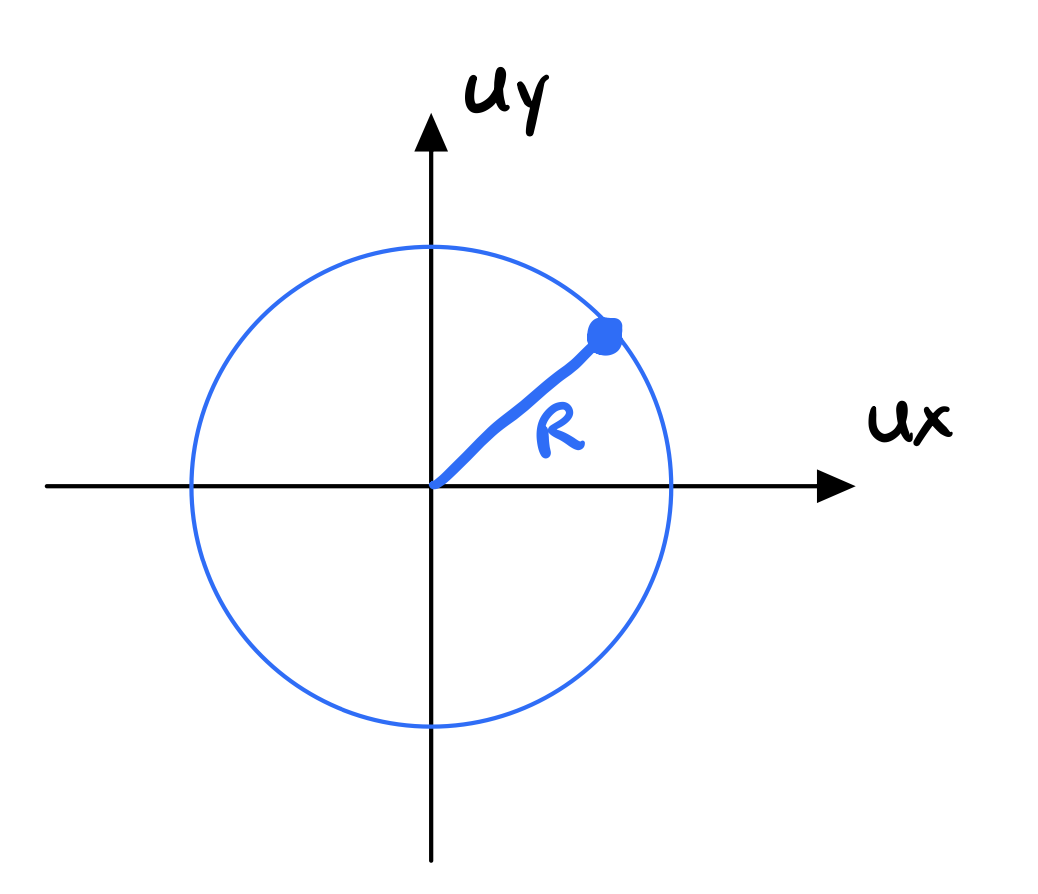
\includegraphics[scale=0.35]{Lectures/Images/lec5-uxuyspace.png}
\end{center}

Then in strain space $(S_1, S_2)$ we have a circle of radius $qR$ will be traced out over one cycle. The work done is (as we have previously calculated):
\begin{equation}
    W_{\text{odd}} = 2K^0 \cdot \text{Area} = 2K^0\pi(qR)^2
\end{equation}
Where does this energy go? We can imagine that this energy is dissipated in each cycle, so that the wave neither dies down, nor does it get amplified without bound. So, let us write down the energy being dissipated, and then balance this with the work done. The dissipated energy is:
\begin{equation}
    W_{\text{dis}} = P\Delta t = \Gamma\abs{\dot{u}}^2T = \Gamma\left(\frac{2\pi R}{T}\right)^2 T = \Gamma (2\pi R)^2 \frac{1}{T} = \Gamma R^2 2\pi \omega
\end{equation}
where $T$ is the period of the cycle. Note in the third equality that we rewrite $\dot{u}$ to be the perimeter divided by the period, and in the last equality we replace $\omega = \frac{2\pi}{T}$. Now, doing an energy balance argument, we say that the energy gained is lost by the dissipation:
\begin{equation}
    W_{\text{odd}} = W_{\text{dis}} \implies 2K^0\pi(qR)^2 = \Gamma R^2 2\pi \omega \implies \boxed{\omega = \frac{K^0}{\Gamma}q^2}
\end{equation}
Note that since the conclusion only tells us that $\omega \sim \frac{K^0}{\Gamma}q^2$ since the heuristic derivation should not necessarily give us the correct prefactor (though it does, here - a more careful derivation gives the same result). 

Note that the wave speed is given by:
\begin{equation}
    c = \frac{K^0 q}{\Gamma}
\end{equation}
so the speed of the wave scales with the wavevector/momentum $q$. Different parts of the spectrum travel at different speeds! Why no square root? We do \emph{not} have an inertial wave, where we would have two time derivatives and hence a $\omega^2$. Instead we have a dispersive wave. Note that if we take $K^0 \to 0$ (the limit of the medium becoming conservative) or take $\Gamma \to \infty$, then the wave speed goes to zero/the waves vanish.

An important note; if we have EoM $\ddot{x} = -kx$, then $k = \frac{\delta^2 U}{\delta x^2}$, we can write it as a variation of the energy. But, given that we have an odd component, $K^0_{ijmn} \neq \frac{\delta \e}{\delta u_{ij}\delta u_{mn}}$, we \emph{cannot} write it as a variation of energy. This is an example of us taking a system of solids - where traditionally everything is written as the variation of an energy - and generalizing it to a dynamical system. The dispersions we will generate as a result will have different character than what we would normally encounter in physics, either classical or quantum.

\subsection{Phonons in damped odd solids - formal argument}
Next, we want to calculate the dispersion relationship formally, and derive the phase diagram to see for what regions/phases in parameter space are phonons stable. We have equation of motion:
\begin{equation}
    \Gamma\p_t u_j = K_{ijmn}\p_i \p_m u_n
\end{equation}
we guess the ansatz:
\begin{equation}
    u_i(\v{x}) =  u_i(\v{q})e^{-i(\v{q} \cdot \v{x} + \omega t)}
\end{equation}
Leaving the algebra as an exercise, we define the parallel and transverse components:
\begin{equation}
    u_\parallel \equiv \hat{q}_i \tilde{u}_i
\end{equation}
\begin{equation}
    u_\perp \equiv \e_{ij}\hat{q}_i \tilde{u}_j
\end{equation}
then the outcome of the exercise would be:
\begin{equation}
    q_i q_m K_{ijmn}\tilde{u}_n = q^2\m{B + G & K^0 \\ -K^0 - A & G}\m{u_\parallel \\ u_\perp}
\end{equation}
If we also write the LHS in terms of $u_\parallel, u_\perp$ then:
\begin{equation}
    -i\omega \Gamma\m{u_\parallel \\ u_\perp} = -q^2\m{B + G & K^0 \\ -K^0 - A & G}\m{u_\parallel \\ u_\perp}
\end{equation}
We can then diagonalize to find the normal frequencies/modes, wherein we shall find:
\begin{equation}
    \omega = -i\left[\frac{B}{2} + G \pm \sqrt{\left(\frac{B}{2}\right)^2 - K^0A  - (K^0)^2}\right]\frac{q^2}{\Gamma}
\end{equation}
Now, the $\frac{B}{2} + G$ term corresponds to an exponential decay. It is proportional to $B, G$. There is something very subtle happening here. We perturb our solid, starting a cycle that generates energy due to $K^0, A$. The bulk and shear moduli $B, G$ do not like the cycles in strain space - from their perspective these cycles cost energy. The presence of the elastic moduli causes the damping of the waves! This is in stark contrast to oscillations that come from a potential, wherein the elastic moduli support the waves.

Going back to our expression for the frequency, the onset of active waves is whenever we have oscillatory motion of the form $e^{\pm i \text{Re}(\omega)t}$. The imaginary component can only give us decay or amplification. To get a real part, we need the square root term to be imaginary. For this, we require that the argument of the square root is negative. Thus the condition for active waves is (defining $\tilde{K}^0 = \frac{2K^0}{B}, \tilde{A} = \frac{2A}{B})$:
\begin{equation}
    \frac{B}{2}\left(1 -  \tilde{K}^0 \tilde{A} - \left(\tilde{K}^0\right)^2\right) < 0
\end{equation}
the phase transition then occurs on the hyperbola:
\begin{equation}
    \tilde{A} = \frac{1}{\tilde{K}^0} - \tilde{K}^0
\end{equation}
so we have the rough phase diagram:

\begin{center}
    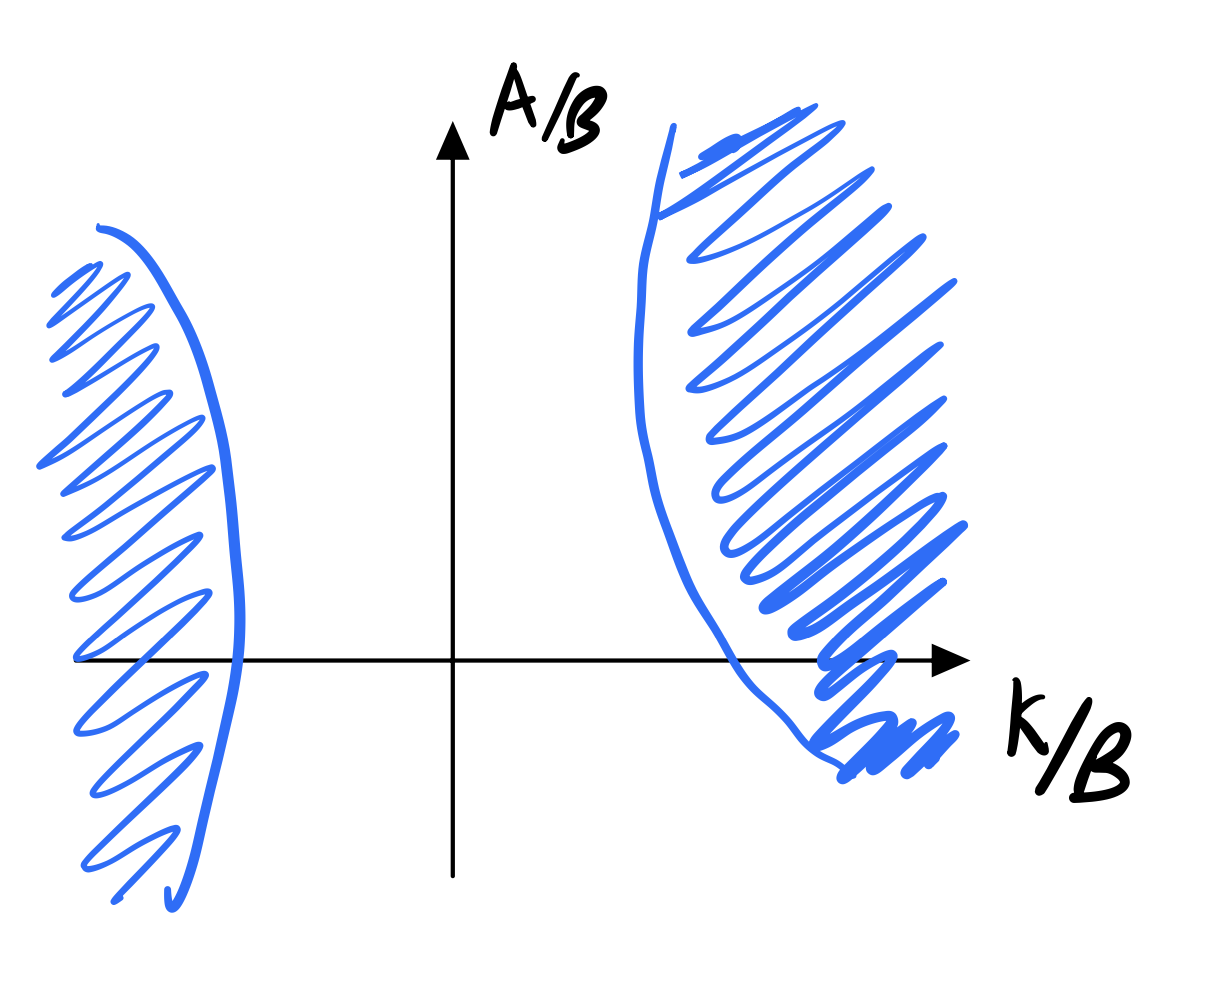
\includegraphics[scale=0.35]{Lectures/Images/lec5-phasediagram.png}
\end{center}

where in the blue regions/phases we get active waves, and in the central condition we have no propagation.

Next class we look at this phase diagram more carefully. We also look at what happens along the $ \tilde{A} = \frac{1}{\tilde{K}^0} - \tilde{K}^0$ lines and look for exceptional points. We also look at limits of large odd elastic moduli and see cases where we have amplification.

\end{document}